\section{Introduction}
\label{sec:intro}

Dense grounded understanding requires models to connect language with fine-grained visual outputs such as pixel-accurate masks over images and videos.
Recent unified systems, such as Sa2VA~\cite{yuan2025sa2va}, move toward this goal by combining a multimodal large language model (MLLM) with a segmentation foundation model, so that a single interface can support both instruction-following conversation and segmentation-oriented prediction.
This unified design is attractive, but also computationally demanding: high-resolution images, long videos, and prompt-conditioned visual evidence all increase the visual token budget before decoding.

Reducing this burden is therefore an important practical problem.
Prior work on visual token compression has shown encouraging results in VQA-style MLLMs, where the main objective is to preserve answer quality under fewer visual tokens~\cite{zhu2025visionselector,yang2024visionzip,zhang2024sparsevlm,zhu2024focusllava,yao2024deco,yang2025topv}.
However, it remains unclear whether the same idea transfers to \emph{dense grounded unified models}.
Compared with VQA, this setting is more sensitive to losing local visual evidence because the model must not only answer questions, but also generate \texttt{[SEG]} tokens that serve as segmentability cues for a downstream mask decoder.
In addition, Sa2VA operates on a unified visual stream containing both image/video tokens and visual-prompt-conditioned tokens, making selection different from ordinary image-token compression in question answering pipelines.

This paper studies a simple question: \emph{can learnable visual token selection remain effective when transferred to a unified image-video model that jointly supports segmentation and conversation?}
We answer this question by equipping Sa2VA with a compatible token selection module and evaluating it on image referring segmentation, video referring segmentation, multimodal conversation, and efficiency profiling.
Our method, \textbf{Sa2VA-Select}, applies token selection to Sa2VA's unified image/video+VP stream after fusion and before the MLLM.
This is the stage where long-context visual evidence and prompt-conditioned evidence first co-exist and jointly affect \texttt{[SEG]} generation.
Rather than redesigning Sa2VA's task interface, we keep its segmentation-and-conversation pipeline unchanged and learn which visual features to retain under a token budget.
Accordingly, Sa2VA-Select is not a new segmentation architecture, but a Sa2VA-compatible transfer of learnable token selection~\cite{zhu2025visionselector} together with a systematic study of when it helps or hurts unified dense grounding.

\begin{figure*}[t]
\centering
\IfFileExists{figure/framework.pdf}{%
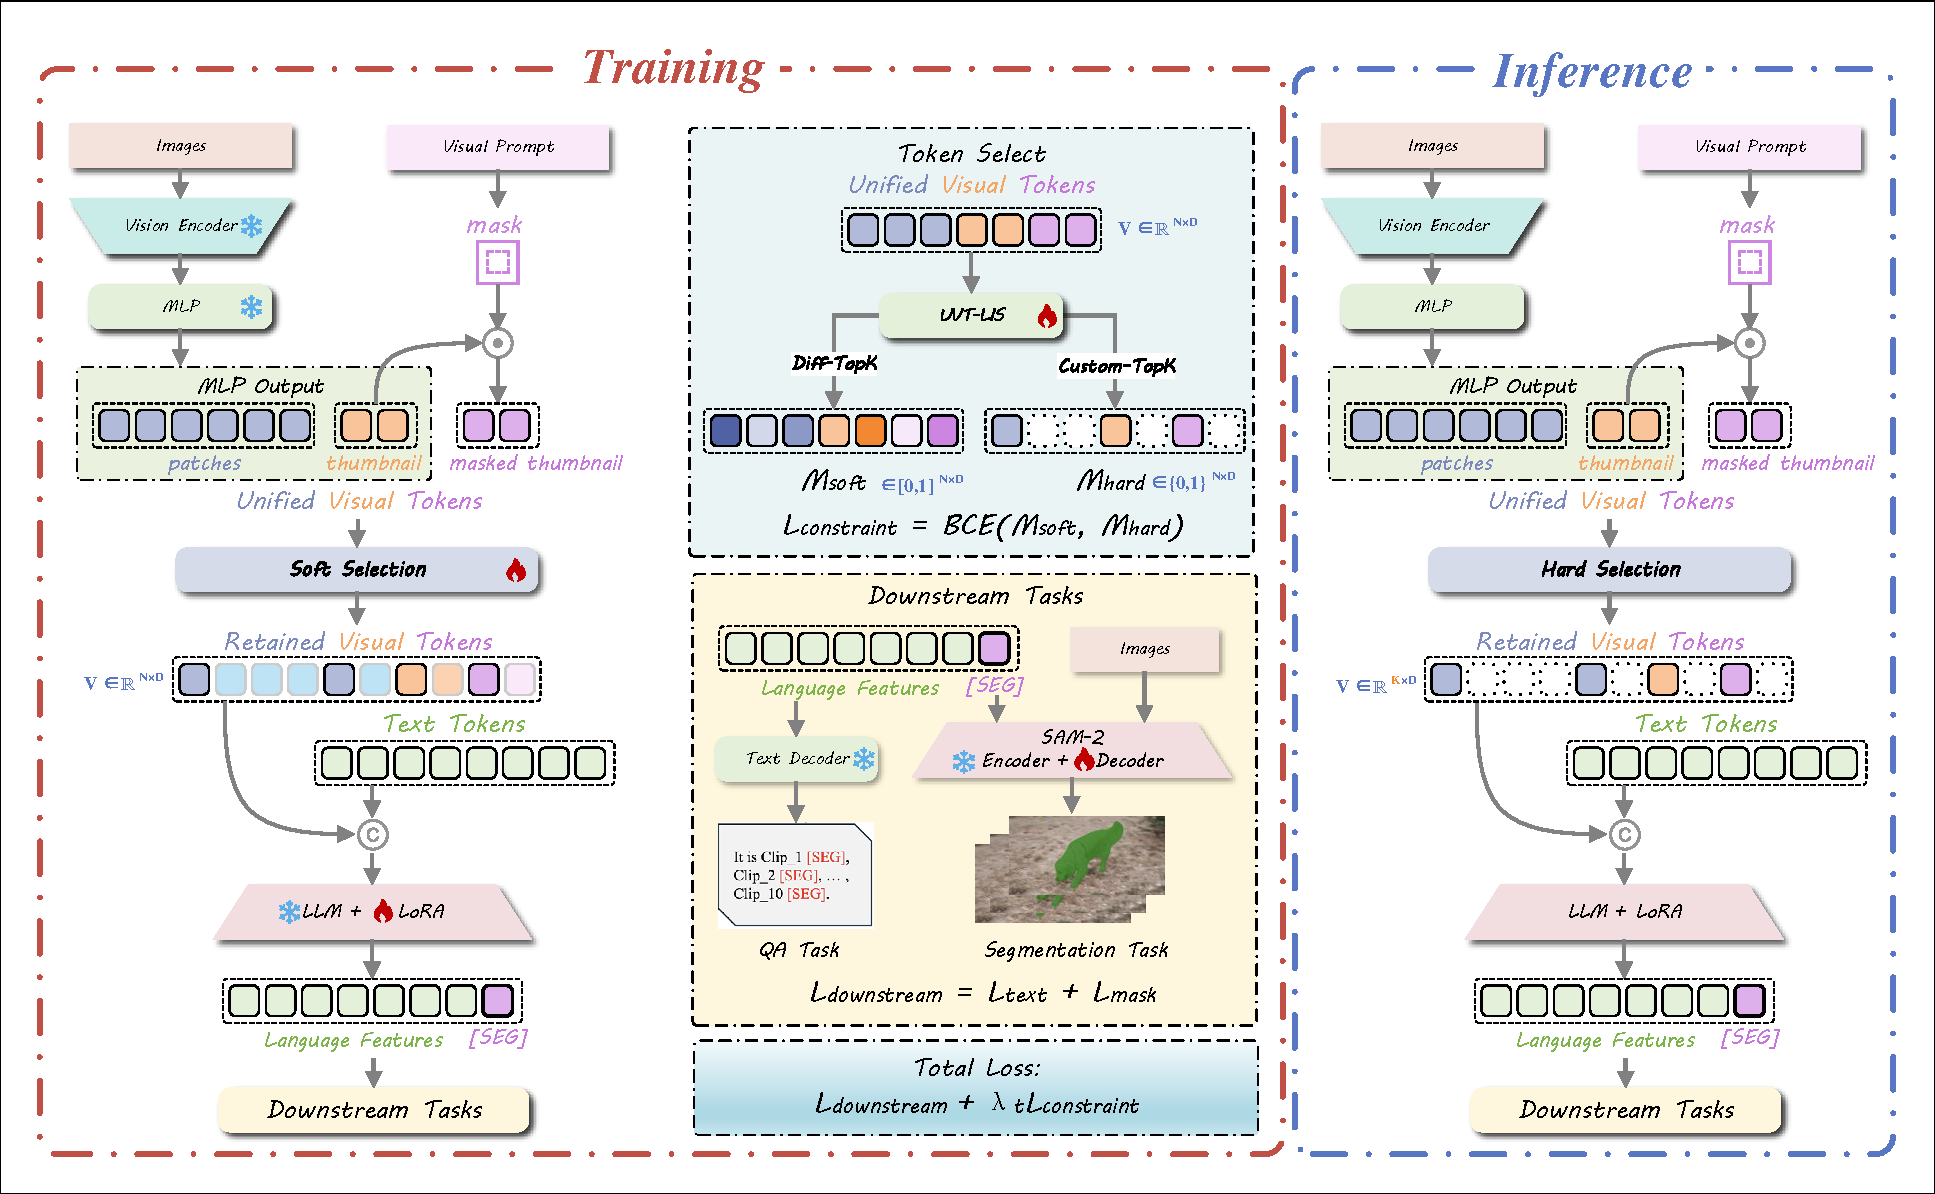
\includegraphics[width=\textwidth]{figure/framework.pdf}%
}{%
\includegraphics[width=\textwidth]{figure/创新图_总.pdf}%
}
\caption{Overall framework of Sa2VA-Select.
	Sa2VA first converts image/video inputs and visual prompts into unified visual tokens.
	We insert a token selection module before the MLLM and apply a Unified Visual Token-oriented Learnable Importance Scorer (UVT-LIS) on the unified visual stream.
	During training, a soft selection branch is optimized with a differentiable Top-$k$ mechanism, while a hard selection branch provides a binary target for the constraint loss, yielding $\mathcal{L}_{\mathrm{constraint}}=\mathrm{BCE}(\mathbf{M}_{\mathrm{soft}}, \mathbf{M}_{\mathrm{hard}})$.
	The retained visual tokens are then concatenated with text tokens for multimodal decoding, supporting both QA and segmentation supervision.
	During inference, we replace soft selection with hard selection to prune low-score visual tokens before the LLM, while keeping Sa2VA's original downstream decoding interface unchanged.}
\label{fig:framework}
\end{figure*}

\paragraph{Challenges.}
Token selection in this setting is non-trivial for three reasons.
First, Sa2VA is inherently multi-task: the retained visual evidence must support both segmentation-oriented supervision and conversation-oriented supervision, which may impose competing demands on the selector.
Second, the visual input is heterogeneous and includes VP-conditioned tokens created from user prompts such as points, boxes, and scribbles; as a result, the selector operates on a \emph{fused} stream rather than on ordinary image tokens alone.
Third, the desired inference operator is hard Top-$k$ pruning for real efficiency gains, but its discreteness introduces a train--test mismatch unless optimization is handled carefully.

\paragraph{Our approach.}
We identify the \emph{unified visual token stream} in Sa2VA as the right intervention point for efficiency.
At this stage, image/video evidence and VP-conditioned evidence have already been assembled, but expensive MLLM decoding has not yet begun.
Sa2VA-Select inserts a budgeted selector here and follows the standard learnable-selection recipe: importance scoring, differentiable budgeted gating during training, and hard Top-$k$ pruning during inference, together with a curriculum constraint that narrows the train--test gap~\cite{zhu2025visionselector,xie2020differentiable}.
This gives a clean test of whether learnable selection can be transferred effectively from VQA-style MLLMs to unified dense grounded understanding through a compatible Sa2VA integration.

\paragraph{Results preview.}
Experiments show that learnable token selection remains effective after being transferred to this more demanding setting.
On Sa2VA-1B, moderate token reduction preserves the baseline's joint segmentation-and-conversation capability, improves several dense grounding benchmarks, and reduces peak GPU memory and prefill time.
Across multiple retention ratios, 30--40\% retention emerges as the preferred operating region.
Qualitative and ablation results further show that the gains are not accidental: the selector reduces distractor-dominant grounding errors, improves temporal stability, and benefits from aligning train-time soft selection with inference-time hard pruning.

\paragraph{Contributions.}
\begin{itemize}
    \item \textbf{Extending learnable token selection to unified dense grounding.} We study how learnable visual token selection transfers to a unified image-video model that jointly supports segmentation and conversation, a setting that is more demanding than prior VQA-style token compression because token pruning must preserve both multimodal reasoning and segmentation-sensitive \texttt{[SEG]} generation.
    \item \textbf{A compatible integration on Sa2VA's unified visual stream.} We place a learnable budgeted selector on the fused image/video+VP token stream before the MLLM, so that token selection can be introduced without redesigning Sa2VA's downstream task interface.
    \item \textbf{Empirical validation of the accuracy--efficiency operating region.} We show across image/video referring segmentation, multimodal conversation, efficiency profiling, qualitative analysis, and ablation studies that moderate token reduction yields the most favorable trade-off region and can even improve dense grounding performance on several benchmarks.
\end{itemize}
